\section{Research Design}

The research follows a design--implement--evaluate methodology. A complete edge-cloud CCTV prototype was implemented first; four evaluation phases were then executed against frozen code and recorded provenance. The phases are: Phase~1, public-dataset probing (CDnet-2014, UCF-Crime); Phase~2, group-aware calibration of the risk score; Phase~3, controlled forensic-integrity testing; and Phase~4, a locked same-codec baseline/SOTA comparison. Protocols are described in this chapter; numerical outcomes are reported exclusively in Chapter~7, so that protocol and result remain separated.

\section{Conceptual Pipeline}

The system implements the following conceptual pipeline:

\begin{center}
CCTV/video source $\rightarrow$ frame capture $\rightarrow$ object detection $\rightarrow$ object/ROI identification $\rightarrow$ risk/state assessment $\rightarrow$ ROI priority assignment $\rightarrow$ adaptive compression and resource allocation $\rightarrow$ encoded stream and event buffer $\rightarrow$ central server $\rightarrow$ dashboard and monitoring.
\end{center}

Each stage is an actually implemented component, not an idealized block. Frame capture and detection run on the edge node; ROI identification merges raw detections with temporal persistence; risk assessment maps ROI content, motion, time of night, scene change, and density into a scalar risk score and a discrete state; allocation converts state and ROI maps into encoder settings; event buffering preserves pre- and post-event context with integrity manifests; the server relays streams and metrics; and the dashboard visualizes them. The following sections define each stage as implemented in \texttt{edge-node/capture\_stream.py}, \texttt{edge-node/detector.py}, and \texttt{evaluation/rate\_allocator.py}.

\begin{figure}[H]
\centering
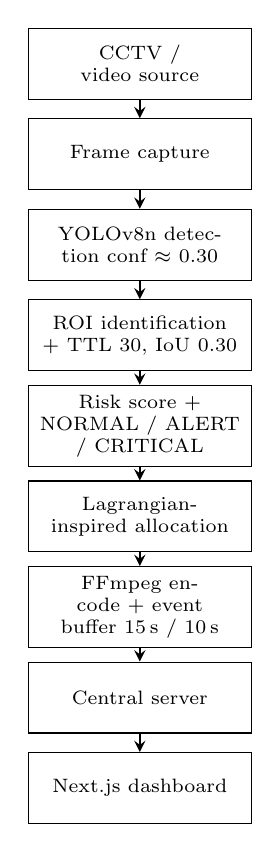
\begin{tikzpicture}[
  node distance=1.15cm, auto,
  block/.style={rectangle, draw, text width=2.6cm, minimum height=0.9cm, align=center, font=\scriptsize},
  arrow/.style={->, >=stealth, thick}
]
\node[block] (src) {CCTV / video source};
\node[block, below of=src] (cap) {Frame capture};
\node[block, below of=cap] (det) {YOLOv8n detection conf $\approx$ 0.30};
\node[block, below of=det] (roi) {ROI identification + TTL 30, IoU 0.30};
\node[block, below of=roi] (risk) {Risk score + NORMAL / ALERT / CRITICAL};
\node[block, below of=risk] (alloc) {Lagrangian-inspired allocation};
\node[block, below of=alloc] (enc) {FFmpeg encode + event buffer 15\,s / 10\,s};
\node[block, below of=enc] (srv) {Central server};
\node[block, below of=srv] (dash) {Next.js dashboard};
\draw[arrow] (src) -- (cap);
\draw[arrow] (cap) -- (det);
\draw[arrow] (det) -- (roi);
\draw[arrow] (roi) -- (risk);
\draw[arrow] (risk) -- (alloc);
\draw[arrow] (alloc) -- (enc);
\draw[arrow] (enc) -- (srv);
\draw[arrow] (srv) -- (dash);
\end{tikzpicture}
\caption{Conceptual pipeline of the implemented system. Each block corresponds to verified code; parameters shown are the evaluated values.}
\label{fig:pipeline}
\end{figure}

[FIGURE PLACEHOLDER --- Figure~1.1 in List of Figures terms: Proposed System Architecture diagram (Edge Node $\rightarrow$ YOLOv8n $\rightarrow$ ROI generation $\rightarrow$ adaptive compression $\rightarrow$ transmission $\rightarrow$ Central Server $\rightarrow$ Dashboard). What to show: deployment-level boxes with data rates and protocols. Purpose: deployment view complementing the pipeline above. Placement: Chapter~5, Section~5.1. Suggested size: 80--90\% of text width. Source: project implementation. Status: NEW FIGURE REQUIRED --- CREATE BEFORE FINAL PRINTING.]

\section{Object Detection and ROI Construction}

Detection uses YOLOv8n (\texttt{edge-node/detector.py}, class \texttt{YoloDetector}, default confidence 0.25 at the API level; 0.30 in all evaluation phases). Detected classes are mapped to priorities by \texttt{priority\_for\_class}: COCO class 0 (person) $\rightarrow$ HIGH; vehicle classes $\{2,3,5,6,7\}$ $\rightarrow$ MEDIUM; all other classes and background $\rightarrow$ LOW. Raw boxes are merged across frames by \texttt{merge\_rois} with IoU threshold 0.30 and smoothing factor 0.4, and each ROI is refreshed with a time-to-live of approximately 30 frames, providing temporal persistence through brief detection gaps. In the Phase~4 comparison, a shared YOLO box cache with 8-pixel dilation was used so that every method operated on identical ROI geometry. Detection is executed on every third frame (\texttt{DETECT\_EVERY\_N} = 3) with CLAHE pre-enhancement when the frame mean falls below 80, and a frame-difference motion fallback fires when no ROI exists but scene change exceeds 0.10.

\section{Risk Scoring and State Assessment}

The heuristic risk score (\texttt{risk\_score} in \texttt{edge-node/capture\_stream.py}) is a weighted sum, capped at 1.0:

\begin{equation}
\mathrm{risk} = \min(1.0,\; 0.30\,n_{\mathrm{HIGH}} + 0.10\,n_{\mathrm{MED}} + 0.03\,n_{\mathrm{LOW}} + 0.25\,\mathrm{motion} + 0.20\,\mathrm{night} + 0.15\,\mathrm{scene} + \min(0.04\,n,\,0.15))
\label{eq:risk}
\end{equation}

where $n_{\mathrm{HIGH}}$, $n_{\mathrm{MED}}$, $n_{\mathrm{LOW}}$ are ROI counts by priority, motion is the normalized frame-difference magnitude, night is a binary indicator (hour $<6$ or $\geq 22$), scene is the scene-change magnitude, and the final term is a density bonus capped at 0.15. The risk score is \textit{primarily a measure of detected-object/ROI importance}; it is not an anomaly probability, and Chapter~7 explains why it must not be read as one. The score drives a three-state machine with hysteresis: risk $\geq$ 0.65 enters CRITICAL; risk $\geq$ 0.30 enters ALERT; CRITICAL exits only below 0.50. States govern compression strength, resolution (640$\times$480 / 854$\times$480 / 1920$\times$1080), GOP structure (120/60, 30/15, 10/5 per state path in the codec manager), and adaptive frame rates.

\section{Lagrangian-Inspired Resource Allocation}

The allocator (\texttt{evaluation/rate\_allocator.py}) distributes a bitrate budget between ROI and background regions. Conceptually, it maximizes a weighted sum of region utilities subject to a total-rate constraint, introducing a Lagrange multiplier $\lambda$ so that each region receives rate $R_i$ satisfying $\partial U_i / \partial R_i = \lambda$; priority weights (HIGH 1.0, MEDIUM 0.4, LOW 0.1) and state-dependent ROI/background budget splits (30/70 NORMAL, 55/45 ALERT, 80/20 CRITICAL) encode ROI importance, and per-ROI rates are clamped to [50, 60\% of ROI budget]. In implementation this is a heuristic solved by a 50-iteration bisection search on $\lambda \in [10^{-6}, 100]$ with tolerance 1.0, using exponential rate--utility models and complexity-adjusted background quality. This thesis therefore describes the method strictly as \textit{Lagrangian-inspired heuristic resource allocation} (a practical approximation), and claims no formally proven global optimality, no convergence guarantee, and no certified optimal bitrate savings. That vocabulary is used consistently throughout the book.

\section{Event Buffering and Forensic Chain}

On entering CRITICAL, the edge node preserves a 15-second pre-event buffer (a frame deque at the operating frame rate) and records a 10-second post-event buffer, dumping frames as JPEG images with per-frame JSON sidecars. After the post-event window completes, \texttt{evaluation/forensic\_chain.py} writes a SHA-256 hash-chained manifest in which each entry links to the previous digest (genesis \texttt{GENESIS}). Verification recomputes digests and chain links over the stored files. The guarantee tested in this thesis is exact-byte integrity behaviour only: recompression, deletion, pixel modification, and sidecar edits are expected to break verification, while untouched evidence is expected to pass. No claim of legal admissibility, certification, or standards compliance is made.

\section{Central Server and Dashboard}

The central server (Node.js/Express with Socket.IO terabits, UDP ingest per camera) relays streams, computes live metrics on a 3-second cadence with automatic bandwidth adaptation, maintains decaying heatmaps, and exposes endpoints for events, motion, cameras, recordings, playback, reconstruction, and 15-second sample requests with real PSNR/SSIM computation. The Next.js dashboard provides live, metrics, playback, and grid views with privacy-mode controls (background blur, face masking, ethical frame-dropping). Details are given in Chapters~5, 6, and 8.

\section{Evaluation Protocols}

\subsection{Phase 1: Public-Dataset Probing}

Protocol (\texttt{evaluation/phase1\_public\_eval.py}): YOLOv8n at confidence 0.30 and 640-pixel width; every 30th frame; frozen risk score; hour fixed to 14 for comparability; CDnet motion threshold 0.0005. CDnet-2014 scenes: \texttt{baseline/highway}, \texttt{baseline/pedestrians}, \texttt{baseline/streetCornerAtNight}. UCF-Crime videos: Normal\_015 and Normal\_050 (normal), Fighting002 (abnormal at clip level; training-split video absent from the supplied annotation pack, so no frame-level evaluation). Burglary001 was excluded because its canonical file could not be verified in isolation; it is documented as not evaluated. Metrics: per-scene risk mean/standard deviation, detection rate, and agreement between detection presence and ground-truth motion inside the temporal ROI; 514 sampled inferences with 0 skipped/failed.

\subsection{Phase 2: Group-Aware Calibration}

Protocol (\texttt{evaluation/phase2\_calibration.py}): 64 labelled seconds (17 positive, 47 negative) from three thesis clips (\texttt{day\_person}, \texttt{day\_empty}, \texttt{night}); labels manually/visually verified with YOLO as assistance only (one night false positive at second 12, a traffic cone, corrected). Model: $P(y{=}1)=\mathrm{sigmoid}(a+b\cdot\mathrm{risk})$ on frozen per-second mean risk, fit with deterministic LBFGS. Splitting: Leave-One-Video-Out (three folds: test on \texttt{day\_empty}, test on \texttt{night}, test on \texttt{day\_person}), plus a full-set descriptive fit. Because all positives come from one video, two test folds are single-class (AUC undefined by construction) and the third train fold is degenerate (zero positives, no fit possible); full-set metrics are therefore apparent/descriptive (in-sample) by construction.

\subsection{Phase 3: Forensic Integrity}

Protocol (\texttt{evaluation/phase3\_forensics.py}): source \texttt{data/thesis\_clips/motion\_only.mp4} (235 frames, 720p); JPEG extraction at quality 2 with JSON sidecars and SHA-256 chain. Five cases with pre-registered expectations: original (expect PASS), clean control (expect PASS), recompressed-vs-original with libx264 CRF 23 (expect FAIL---exact-byte hashes are fragile to transcoding, so this FAIL is a predicted bound, not an experiment failure), recompressed-own-manifest (expect PASS), tampered-vs-pristine with blackout boxes on frames 50/100/150, deletion of \texttt{ev\_00200.jpg}, and sidecar edit of \texttt{ev\_00100\_meta.json} (expect FAIL with localization). Metrics: files checked, missing, hash mismatches, chain mismatches, first failure, localization precision/recall, and clean-case false alarms.

\subsection{Phase 4: Locked Baseline Comparison}

Protocol (\texttt{evaluation/phase4\_sota.py}): primary clip \texttt{motion\_only.mp4} (720p, 235 frames); control clip \texttt{day\_empty.mp4} (777 frames, no ROI); four methods (A uniform, B ROI-QP, C foreground/background split with frozen frame-0 background at 0.5$\times$, D proposed adaptive ROI); bitrate targets 300/600/1200/2400 kbps primary and 300/1200 kbps control; identical source, resolution, frame count, GOP 60 (keyint minimum 30), medium preset, libx265 throughout; one shared YOLOv8n pass per source frame at confidence 0.30 cached to JSON, with 8-pixel dilation and union masks computed from source boxes only (never from encoder outputs); risk thresholds 0.30/0.65 without hysteresis (documented deviation from the live system); background scales 0.25 (B), 0.35/0.60/1.00 by state (D). Metrics: actual bitrate, PSNR/SSIM globally and over ROI/background masks, and detector consistency (recount with the same YOLO on outputs---an internal-consistency check, not independent detection accuracy). BD-rate is reported only if at least four overlapping points, at least 1\,dB of shared interval, and clean fits hold for all comparisons; otherwise it is withheld. Runtime was approximately 3.5 hours wall-clock (9764\,s) on the CPU-only machine.
